\subsection{Context-Aware Scene Prediction}
\label{ssec:caspnet}

This section distills the key ideas behind \emph{Context-Aware Scene Prediction Network} (CASPNet)~\cite{caspnetSchäfer2022} and its transformer successor \emph{CASPFormer}~\cite{caspformerYadav2024}. Both architectures perform \emph{joint multi-agent} trajectory forecasting from rasterized bird's-eye-view (BEV) inputs, yet they differ strongly in how they fuse context and decode trajectories. We summarize their core components, strengths, and limitations.

\subsubsection*{CASPNet: Rasterized BEV Encoding with Dual FPN}

\textbf{CASPNet}~\cite{caspnetSchäfer2022} processes rasterized BEV inputs through a dual-encoder architecture that separately handles dynamic agent trajectories and static HD map information. Overall, it strongly resembles a \emph{fully convolutional network} as it employs no fully connected layers, meaning that the spatial representation of the scene is preserved throughout the network. Furthermore, it can be classified as a \emph{feature pyramid network} (FPN)~\cite{FPNLin2017} as it provides the decoder with latent representations at multiple spatial resolutions. Together, these architectural qualities starkly resemble the famous \emph{U-Net} architecture with \emph{lateral skip connections}~\cite{UNetLSRonneberger2015}. Considering CASPNet's usage of \emph{attention} mechanisms within the skip connections its closest relative in the field of image segmentation is the \emph{Attention U-Net}~\cite{UNetAttnOktay2018}.

\begin{figure}[ht]
  \centering
  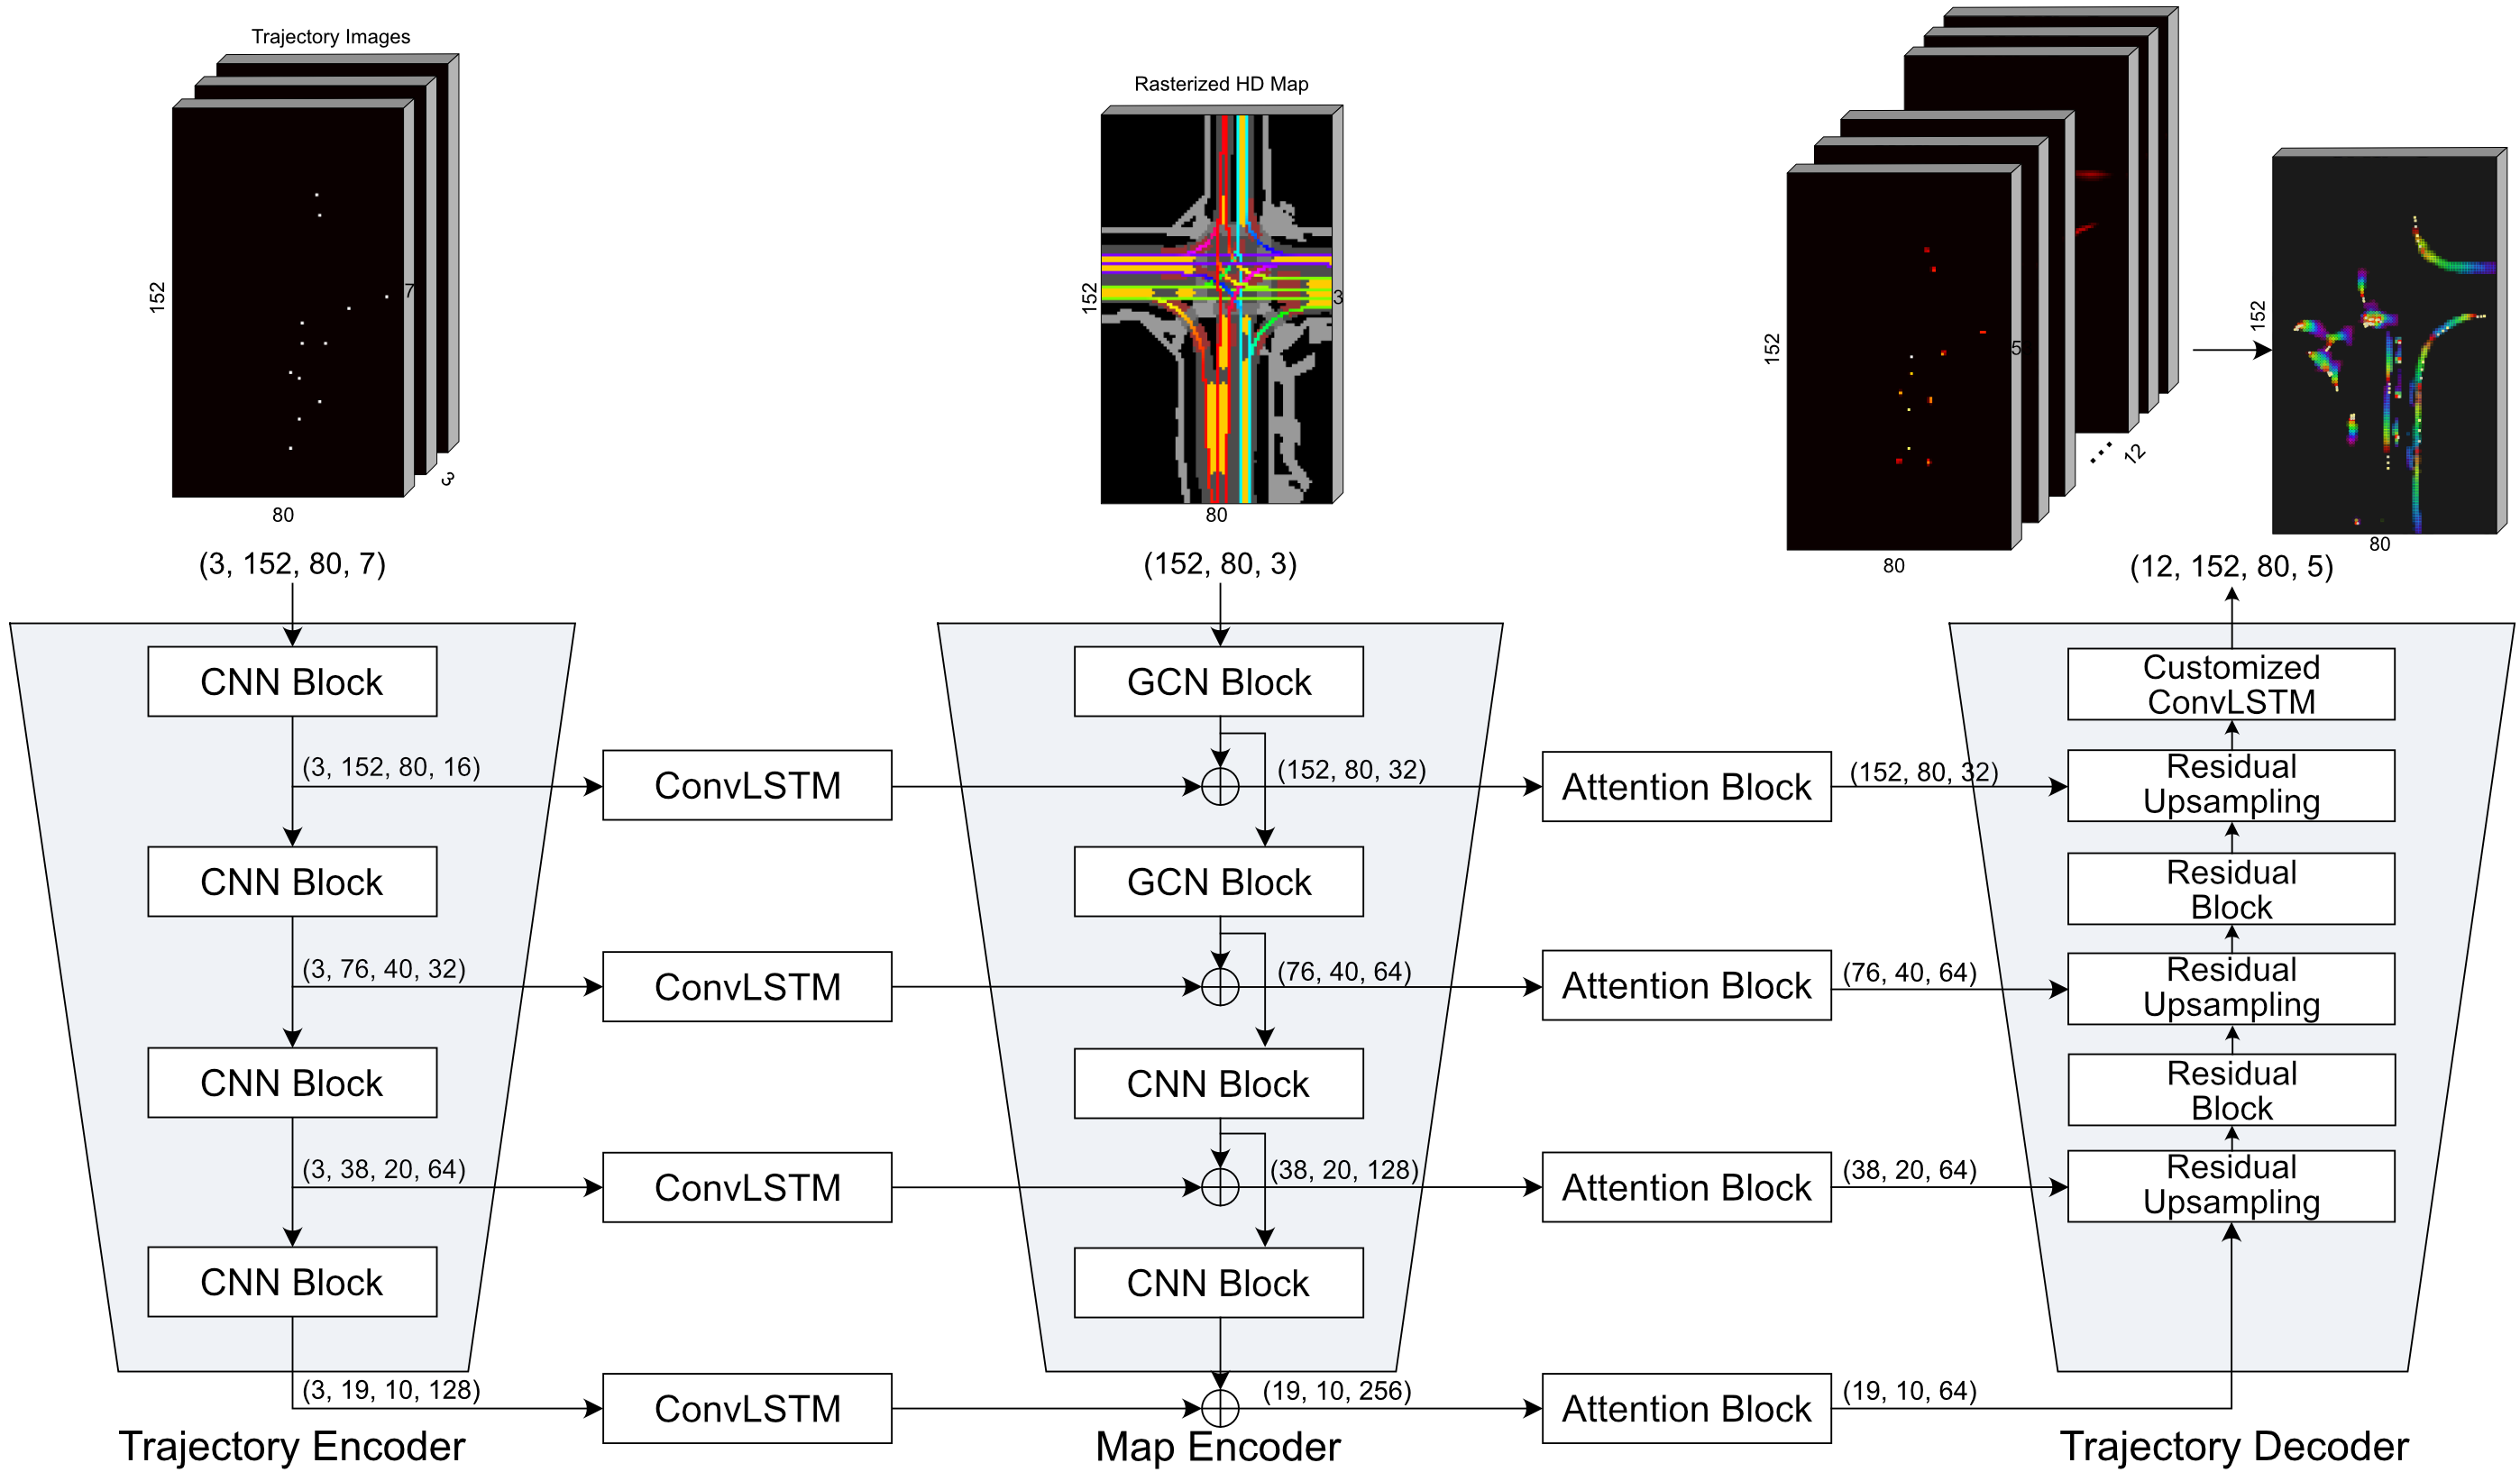
\includegraphics[width=\linewidth]{figures/caspnet_arch.png}
  \caption{CASPNet architecture overview: dual FPN encoders with Gabor filters, pixel-adaptive attention, and grid-based ConvLSTM decoder~\cite{caspnetSchäfer2022}.}
  \label{fig:caspnet_overview}
\end{figure}

The CASPNet architecture is illustrated in~\autoref{fig:caspnet_overview} and consists of the following components:
\begin{description}[leftmargin=1em,itemsep=2pt]
\item[Dual FPN encoders.] Separate feature-pyramid networks process
\begin{enumerate}[label=\roman*)]
    \item a BEV stack of past agent trajectories \( \mathbf{I}_d\in\R^{T_p\times H\times W\times F_d} \)
    \item a static HD-map raster \( \mathbf{I}_s\in\R^{H\times W\times F_s} \)
\end{enumerate}

At each level \( \ell \), the trajectory branch produces:
\begin{equation}
\label{eq:fpn_traj}
\mathbf{F}^{\mathrm{traj}}_{\ell}(t) = \mathrm{CNN}_\ell\bigl(\mathbf{I}_{d}(t)\bigr) \in \R^{T_p \times C_\ell \times H_\ell \times W_\ell}
\end{equation}
where all \( T_p \) BEV frames representing the agent trajectories are encoded independently by the same CNN, yielding a \emph{time-dependent} \emph{multi-scale feature map} \( F^{\mathrm{traj}}_{\ell}(t) \in \R^{C_\ell \times H_\ell \times W_\ell} \) at each pyramid level \(\ell\) and timestep \( t \in \{0,\dots,T_p - 1\} \).\\

The static map branch employs \emph{steerable Gabor filters}%
\footnote{See~\autoref{ssec:gabor_filters} for further details.}
in the first two convolutional blocks. These filters are particularly well-suited for capturing orientation and scale-sensitive features like road networks, where lane markings exhibit strong orientation and scale-specific patterns. A Gabor filter combines a Gaussian envelope with a sinusoidal carrier wave, allowing it to simultaneously localize features in space and frequency. This makes it highly effective for detecting elongated and parallel structures across varying scales and rotations~\cite{steerableGaborFilters}.\\
The map features are computed as follows:
\begin{equation}
\label{eq:fpn_map}
\mathbf{F}_{\ell}^{\mathrm{map}}
= \mathrm{CNN}_\ell^{\circ}(\mathbf{I}_s) \in \R^{C_\ell \times H_\ell \times W_\ell},
\end{equation}

\item[Temporal fusion.] ConvLSTM cells at every pyramid level aggregate the temporal context across all \(T_p\) timesteps yielding a single feature map per level~\cite{shi2015ConvLSTM}:
\begin{equation}
\label{eq:fpn_fusion_traj}
\mathbf{F}_{\ell}^{\mathrm{traj}}
= \mathrm{ConvLSTM}_\ell\Bigl\{\mathbf{F}^{\ell}_{d}(t)\Bigr\}_{t=1}^{T_p} \in \R^{C_\ell \times H_\ell \times W_\ell},
\end{equation}
which are then concatenated with the static map features at each level:
\begin{equation}
\label{eq:fpn_fusion}
\boldsymbol{\mathcal{F}}=\{\mathbf{F}_\ell^{\mathrm{traj}}\oplus \mathbf{F}_\ell^{\mathrm{map}}\}_{\ell=0}^{L_{\text{FPN}}-1}, \quad \text{where } \mathbf{F}_\ell \in \R^{2 C_\ell \times H_\ell \times W_\ell}
\end{equation}
\( \boldsymbol{\mathcal{F}} \) is the resulting latent feature pyramid.

\item[Pixel-adaptive attention.] The \emph{Attention Block} in the lateral skip connections (\autoref{fig:caspnet_overview}) adaptively blends the receptive fields of multiple \emph{dilated convolutions}~\cite{dilatedConv21} per spatial location, capturing multi-scale interactions through learned per-pixel attention weights over different dilation rates, similar to~\cite{UNetAttnOktay2018}. For each location \((i,j)\) at pyramid level \(\ell\), the mechanism computes:
\begin{equation}
\label{eq:pixel_attention}
\mathbf{F}_{\ell}^{(i,j)} = \sum_{r} \alpha^{(i,j)}_{r} \cdot \text{DilatedConv}_r(\mathbf{F}^{(i,j)}_{\ell}),
\end{equation}
where \(\alpha^{(i,j)}_{r} = \text{softmax}(\text{Conv}(\mathbf{F}^{(i,j)}_{\ell}))\) are learned attention weights that dynamically select appropriate receptive field sizes for each spatial location.

\item[Grid-based decoder.] The decoder employs a series of \emph{residual up-sampling blocks} to progressively up-sample the feature maps from the FPN to the original raster resolution. Each residual block consists of a parallel \emph{transposed convolution} and a \emph{linear interpolation} layer. The resulting feature maps of each up-sampling block are concatenated with the corresponding feature maps the next level of the FPN.\\
Finally, the decoder uses a \emph{ConvLSTM} layer to autoregressively generate future predictions. For each future timestep \(t \in \{T_p, \ldots, T_p + T_f - 1\}\), the decoder outputs a occupancy probabilities and motion offsets. The occupancy probabilities are represented as a categorical distribution over the possible agent classes at each pixel, while the motion offsets represent the displacement of each pixel with respect to the previous timestep~\cite{caspnetSchäfer2022}.

\paragraph{Pros.} Inference time independent of agent count; inherent multi-modality via heat-map superposition; good interpretability through adaptation of well-established motifs from the field of image segmentation.
\paragraph{Cons.} Metric accuracy capped by raster resolution; inference cost scales with grid size; vectorized outputs require post-processing; no \emph{explicit} prediction of \( M \) multi-modal; doesn't respect identities of agents; limited temporal modeling; no explicit relationship modeling between agents or between agents and map; no symmetries in the agent-centric coordinate system for all but the ego agent; only suited for \emph{single-agent} motion forecasting.

The follow-up work CASPNet++~\cite{caspnetppSchäfer2023} improves upon CASPNet by replacing its single heat-map head with a two-stage design to capture spatio-temporal occupancy grids for every actor, as well as an Agent decoder that transforms the grid cells of selected targets into explicit, multi-modal trajectory splines, thereby modelling interactions more richly and introducing the ability to predict \( M \) explicit multi-modal trajectories. However, while CASPNet++ improves upon the original architecture in terms of accuracy and interaction modeling and allows for \emph{true} joint multi-agent forecasts, we will not discuss it in detail.

%--------------------------------------------------------------------
%% Above is done %%
\subsubsection*{CASPFormer: Hybrid CNN-Transformer with Deformable Attention}
\label{ssec:caspformer}

\textbf{CASPFormer}~\cite{caspformerYadav2024} retains CASPNet's, FPN-CNN backbone while replacing its grid-based decoder with a transformer that emits vectorized \((x,y)\) trajectories, explicitly modeling the uncertainties of each mode as a \emph{parametrized Laplacian}. The core innovation lies in adapting \emph{deformable attention}~\cite{zhu2021deformabledetr} from object detection to trajectory prediction, enabling sparse, efficient attention over multi-scale feature representations. The overall architecture is illustrated in~\autoref{fig:caspformer_overall}, with the detailed decoder mechanism shown in~\autoref{fig:caspformer_decoder}. The following section requires basic understanding of both regular and deformable attention mechanisms. While we are referring the reader to~\cite{vaswani2023attention} and~\cite{zhu2021deformabledetr} for a detailed introduction, a concise explanation of the key concepts is provided in \autoref{sec:deformable_attention}.

\begin{figure}[ht]
  \centering
  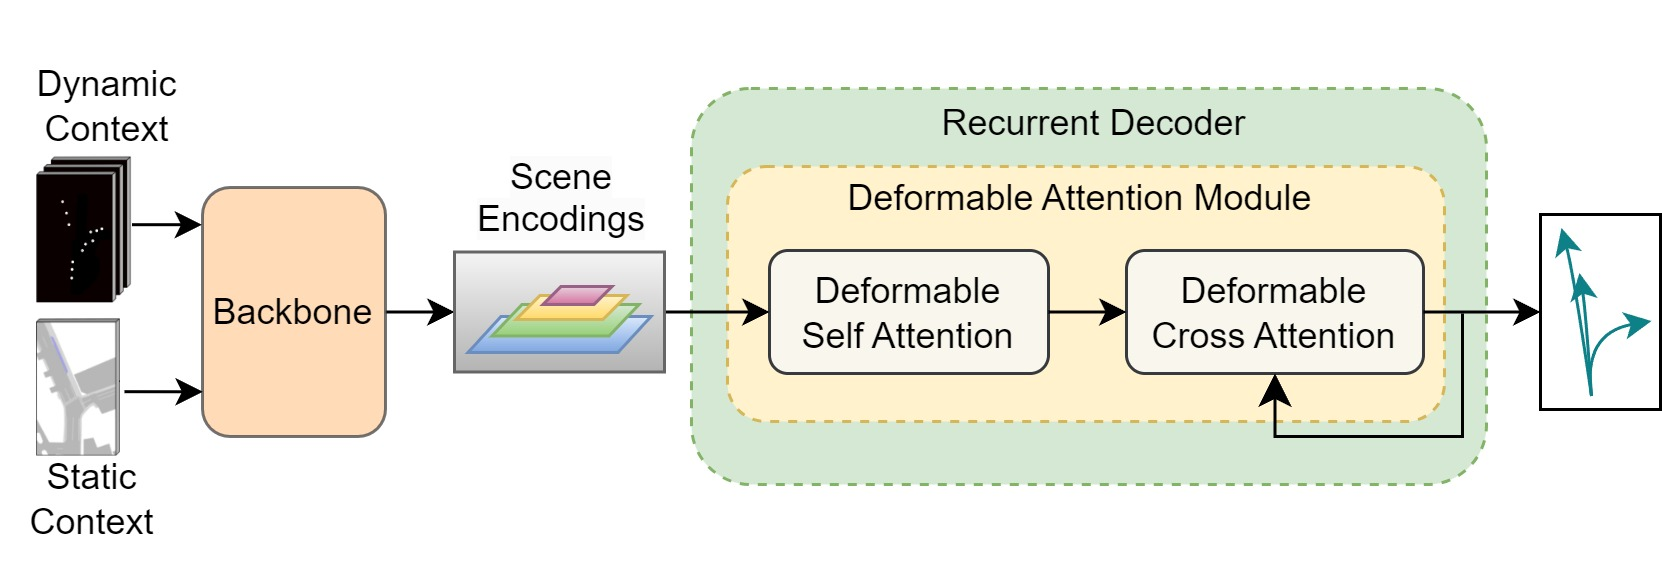
\includegraphics[width=\linewidth]{figures/caspformer-overall-arch.jpg}
  \caption{CASPFormer overall architecture: CNN+FPN backbone processes rasterized BEV inputs, deformable self-attention fuses multi-scale features, and recurrent deformable cross-attention autoregressively decodes vectorized trajectories~\cite{caspformerYadav2024}.}
  \label{fig:caspformer_overall}
\end{figure}

\begin{figure}[ht]
  \centering
  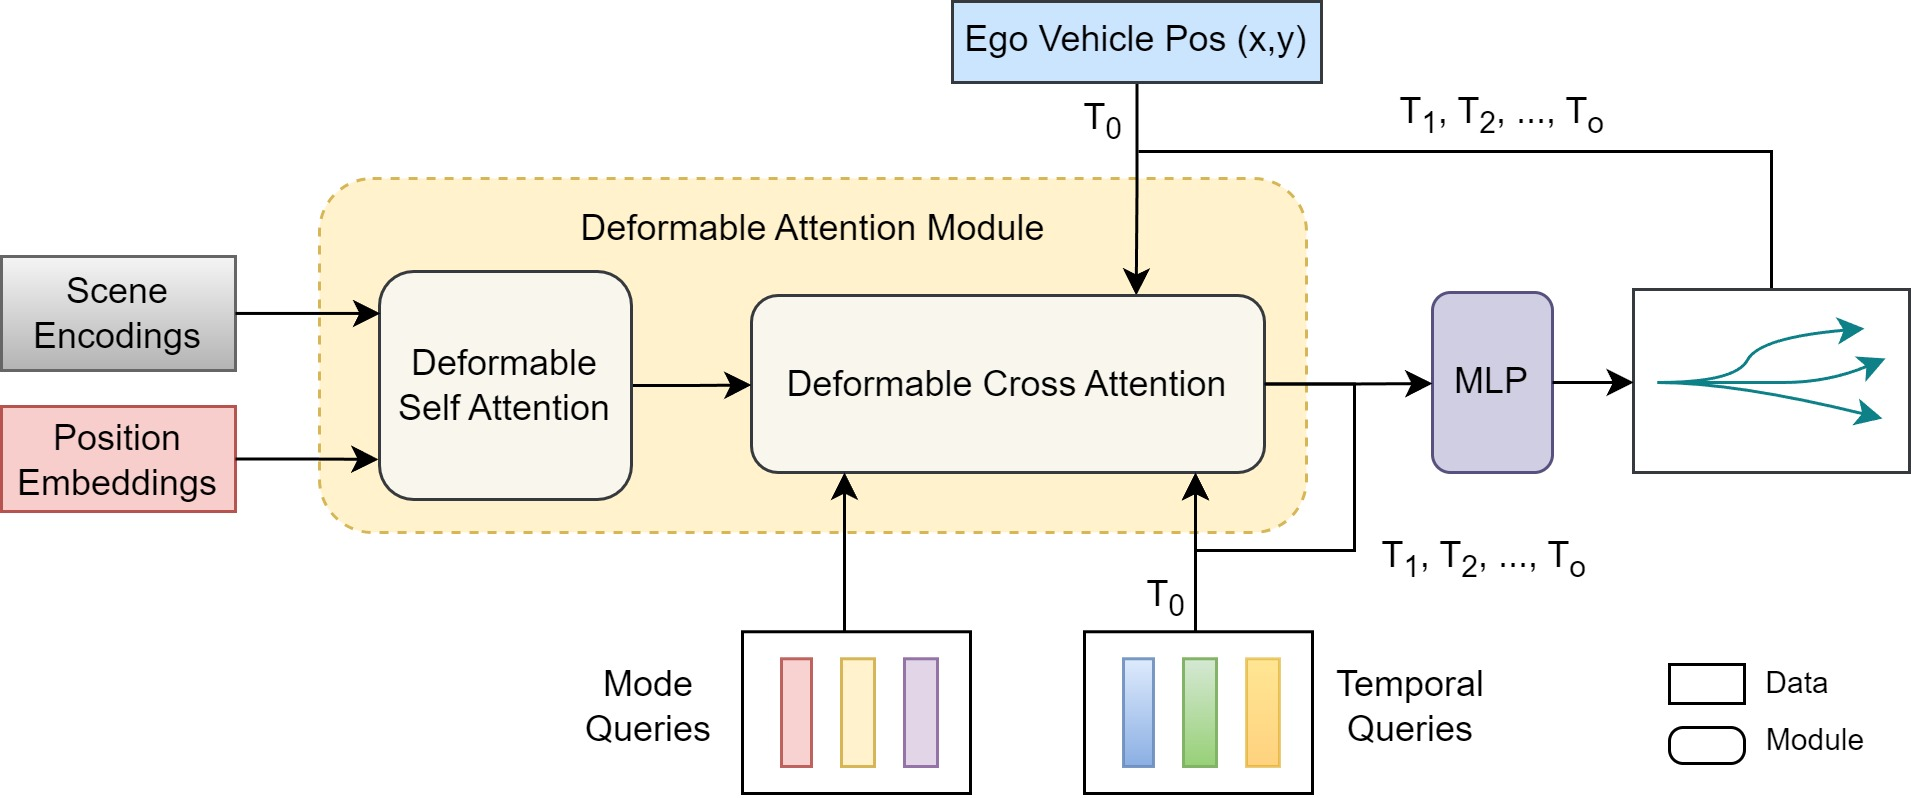
\includegraphics[width=0.85\linewidth]{figures/caspformer_decoder.jpg}
  \caption{CASPFormer decoder architecture with temporal and mode queries, deformable cross-attention, and autoregressive trajectory generation~\cite{caspformerYadav2024}.}
  \label{fig:caspformer_decoder}
\end{figure}

The CASPFormer as depicted in \autoref{fig:caspformer_decoder} decoder consists of the following key components:

\begin{description}[leftmargin=1em,itemsep=2pt]
\item[Multi-Scale Deformable Self-Attention (MSDA).] The FPN feature maps \(\boldsymbol{\mathcal{F}} = \{\mathbf{F}_\ell\}_{\ell=0}^{L-1}\) as previously defined in \autoref{eq:fpn_fusion} are first flattened and enriched with non-learnable 2D sinusoidal positional encodings as introduced in~\cite{vaswani2023attention} to preserve spatial relationships across different scales. MSDA performs feature fusion by allowing each spatial location to attend to relevant features across all pyramid levels:

\begin{equation}
\label{eq:msda_operation}
\mathbf{Z}^{\text{SA}} = \sum_{n=1}^{N_H} \mathbf{W}_{n} \left[\sum_{\ell=0}^{L_{\text{FPN}}-1} \sum_{k=1}^{K_s} A_{n\ell qk} \cdot \mathbf{F}_\ell(\phi_{\ell}(\mathbf{p}_q) + \boldsymbol{\Delta p}_{n\ell qk}) \right]
\end{equation}

Here, \emph{queries} and \emph{keys} are derived from the same flattened feature maps \(\text{Flatten}(\boldsymbol{\mathcal{F}} + \textbf{PE})\). The learned offsets \(\boldsymbol{\Delta p}_{\ell nkq} \in \R^2\) enable each query to attend to informative locations across the entire feature pyramid, while being constrained to all features of the n-th attention head. \( \phi_{\ell} \) re-scales the normalized coordinates \( \mathbf{p}_q \in [0,1]^2\) to the spatial dimensions of the feature map at level \(\ell\).\\
  The output of the MSDA is a latent representation of the entire scene, encoding all spatio-temproal and social dynamics of the agents and the map. Hence, this module should be seen as part of the scene-encoder, rather than the decoder.

\item[Recurrent Deformable Cross-Attention.] The fused features \(\mathbf{Z}^{\text{SA}}\) serve as \emph{keys} and \emph{values} for the cross-attention mechanism. CASPFormer employs a dual-query approach that combines \emph{temporal queries} and \emph{mode queries} to capture both temporal dependencies and facilitate mode diversity. The query construction is defined as:

\begin{equation}
\label{eq:dual_query_construction}
\begin{aligned}
\mathbf{Q}_t^{\text{temp}} &= \mathbbm{1}(t=T_p) \cdot \mathbf{E}_{\text{init}} + \mathbbm{1}(t>T_p) \cdot \mathbf{Z}^{\text{CA}}_{t-1} \\
\mathbf{Q}^{mode} &\in \R^{M \times d} \quad \text{(learnable mode embeddings)} \\
\mathbf{Q}_t &= \mathbf{Q}_t^{temp} \oplus \mathbf{Q}^{mode} \quad \text{(concatenated dual queries)}
\end{aligned}
\end{equation}

The temporal queries maintain temporal coherence across timesteps, while mode queries provide fixed embeddings to promote behavioral diversity and mitigate mode collapse.

For each timestep \(t\), the deformable cross-attention decoder updates the reference point \(\mathbf{p}^{ref}\) as the last position of the ego-vehicle \( \hat{\boldsymbol{\mu}}_{t-1}\) based on previous predictions and computes:
\begin{equation}
\label{eq:cross_attention_operation}
\mathbf{Z}^{\text{CA}}_t = \sum_{m=1}^{M} \mathbf{W}_m \left[ \sum_{k=1}^{K_s} A_{nkq} \cdot \mathbf{Z}^{\text{CA}}(\mathbf{p}^{ref} + \boldsymbol{\Delta p}_{nkq}) \right]
\end{equation}

where both the attention weights and offsets are computed as delineated in~\autoref{sec:deformable_attention}. The DCA block depicted in~\autoref{fig:caspformer_decoder} stacks three deformable cross-attention layers, each with its own set of learnable parameters, to refine the predictions iteratively. This allows the model to capture complex interactions and dependencies across multiple timesteps and modes.

\item[Autoregressive Decoding with Mixture Outputs.] The outputs of the final cross-attention layer are processed by an MLP to generate trajectory distributions as mixtures of Laplacian components:
\begin{equation}
\label{eq:mixture_trajectory_output}
\begin{aligned}
\hat{\boldsymbol{\mu}}_{t}, \hat{\mathbf{b}}_{t} &= \text{MLP}(\mathbf{Z}^{\text{CA}}_t)\\
\hat{\boldsymbol{\pi}} &= \text{softmax}(\text{MLP}(\mathbf{Z}^{\text{CA}}_t)) \\
\end{aligned}
\end{equation}
where \(\hat{\boldsymbol{\mu}}_{t} \in \R^{N_c \times M \times 2}\) are Cartesian position means, \(\hat{\mathbf{b}}_{t} \in \R^{N_c \times M \times 2}\) are uncertainty scales, and \(\hat{\boldsymbol{\pi}}_t \in \R^{N_c \times M}\) are mode probabilities for each of the \(M\) trajectory modes and each agent of interest; \( N_c \) being the number of agents in the scene, whose trajectories are to be predicted.

The recurrent architecture updates both the temporal queries and reference point at each timestep:
\begin{equation}
\label{eq:recurrent_updates}
\begin{aligned}
\mathbf{p}^{ref}_{(t+1)} &= \text{argmax}_m \hat{\boldsymbol{\pi}}_{t,ego} \cdot \hat{\boldsymbol{\mu}}_{t,m^{ego}} \\
\end{aligned}
\end{equation}
where \(m^* = \text{argmax}_m \hat{\boldsymbol{\pi}}_{t,ego}\) yields the index of the ego agent's most probable mode, hence the next reference point is set the likeliest predicted position of the ego vehicle (which must be one of the \( N_c \) agents of interest).
\end{description}

\paragraph{Loss Formulation and Training Recipe.} CASPFormer adopts the HiVT loss formulation~\cite{zhou2022hivt}, combining regression and classification objectives \(\mathcal{L} = \mathcal{L}_{reg} + \mathcal{L}_{cls}\).\\
The regression loss optimizes the mode with the lowest Euclidean distance to the ground truth trajectory of each agent, to encourage diverse trajectory predictions:
\begin{equation}
  \label{eq:caspformer_regression_loss}
  \mathcal{L}_{reg} = -\frac{1}{T_f} \sum_{t=1}^{T_f} \log[\mathbb{L}(P_t \mid \mu_t, b_t)]
\end{equation}
The influence of all other modes and the predicted categorical distribution is captured by a cross-entropy classification loss:
\begin{equation}
  \label{eq:caspformer_classification_loss}
  \mathcal{L}_{cls} = -\frac{1}{M} \sum_{k=1}^{M} \log(\pi_k) \mathbb{L}(P_{T_f, k} \mid \mu_{T_f, k}, b_{T_f, k})
\end{equation}
\end{description}

\paragraph{Pros.} Direct vectorized output without post-processing; explicit multi-modal prediction and uncertainty estimates; deformable attention enables efficient Transformer decoding; Using the past-predictions as temporal queries introduces grounding and interpretability; complexity scales with the number of agents \( N_c \), not grid size \(\mathcal{O}(HW)\); mode-queries mitigate mode collapse.

\paragraph{Cons.} Still inherits quantization artifacts from the rasterized backbone; limited to ego-agent-centric coordinate systems; BEV raster discretization artifacts in crowded intersections; memory overhead for large \(H \times W\) grids.

% \paragraph{Empirical Performance and Limitations.} On nuScenes validation, CASPFormer achieves 1.23m minFDE and 2.85m minADE, representing 30--40\% improvement over CASPNet while maintaining real-time inference at \(\sim\)20 FPS on V100 GPUs. The deformable attention mechanism reduces computational complexity from \(\mathcal{O}(H \cdot W \cdot T_f)\) for grid-based approaches to \(\mathcal{O}(M K_s \cdot T_f)\) where \(M K_s \ll H \cdot W\) represents the decoder complexity with \(M = 5\) modes and \(K_s = 4\) sampling points per query.

% However, CASPFormer inherits certain limitations from its rasterized backbone. The BEV rasterization process can introduce sparse artifacts in regions with limited map coverage, affecting prediction quality in complex intersections or areas with irregular geometry. Additionally, failure cases include scenarios with highly dynamic pedestrians in dense crowds and abrupt lane-change maneuvers that exceed the temporal modeling capacity of the recurrent decoder. Unlike CASPNet, which outputs discrete grid-based likelihood distributions that can be directly interpreted as trajectory modes, CASPFormer generates continuous trajectory coordinates through mixture distributions but does not provide explicit trajectory mode probabilities in the same interpretable format.

% The key innovation lies in the dual-query architecture that addresses mode collapse while maintaining temporal consistency. Unlike single-query approaches that struggle with behavioral diversity, the separation of temporal and mode queries enables CASPFormer to generate distinct trajectory modes while preserving smooth temporal dynamics.

%--------------------------------------------------------------------
\newpage